\section{\textit{Optimisation II} \er{NO\_SolInit3}}
The goal of this program is ...



\begin{figure}[h!]
\centering
\begin{tikzpicture} 
\node (start) at (0,0) [call] {TestLib NO\_SolInit3}; 
\node (main) at (0,-2) [process] {CPP\_NewSolGolInit\_main};


\draw [arrow] (start) --  (main);    

\end{tikzpicture}
\caption{Triplet optimisation II workflow.}\label{fig:workfOptim2}
\end{figure}


\subsection{Main classes, some typedefs and variables}
\begin{itemize}
\item $cAppli\_NewSolGolInit$ -- the manager class
\item $cRandNParmiQ$ -- class for random selections
\item $cNOSolIn\_AttrSom$ -- class corresponding to a node, defined in SolInitNewOri.h
\item $cNOSolIn\_AttrArc$ -- class corresponding to an edge, defined in SolInitNewOri.h
\item $cNOSolIn\_Triplet$ -- triplet solution 
\item $cLinkTripl$ -- it is an ordered  $cNOSolIn\_Triplet$

\item[--] $typedef  ElSomIterator<cNOSolIn\_AttrSom,cNOSolIn\_AttrArc> tItSNSI$ -- iterator over nodes
\item[--] $typedef  ElArcIterator<cNOSolIn\_AttrSom,cNOSolIn\_AttrArc> tItANSI$ -- iterator over arcs
\end{itemize}


\subsection{Algorithms} 

%%%%%%%%%%%%%%%%%%%%%%%%%%%%%%%%%%%%%%%%%%  cAppli_NewSolGolInit::cAppli_NewSolGolInit
\begin{algorithm}
\caption{\er{$cAppli\_NewSolGolInit::cAppli_NewSolGolInit$}; def in cNewO\_SolGlobInit.cpp  }
\begin{algorithmic}
\State 
\\
\Comment \cmt{Load the graph, i.e. all the nodes/images and the edges : mMapS, mGr and  mV3}
\\
\\
\Comment \cmt{Calculate an average coherence score for each triplet. }
\State $EstimCoherenceMed();$
\\
\\
\Comment \cmt{Estimate robust rotations from available triplets }
\State $EstimRotsArcsInit();$
\\
\\
\Comment \cmt{dd }
\State $EstimCoheTriplet();$
\\
\\
\Comment \cmt{dd }
\State $FilterTripletValide();$
\\
\\
\Comment \cmt{dd }
\State $mTestTrip->CalcCoherFromArcs(true);$
\\
\\
\Comment \cmt{dd }
\State $NumeroteCC();$
\\
\\
\Comment \cmt{dd }
\State $CalculOrient();$
\\ 

\end{algorithmic}\label{alg:Optim2}
\end{algorithm}


\begin{figure}
\centering
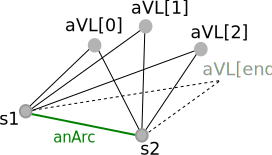
\includegraphics[width=7cm]{img/triplet-sel.pdf}\caption{Illustration to Alg.~\ref{alg:Optim2CohMed}. The coherence scores are calculated for all combinations of triplets, e.g. a couple of triplet $s1-s2-aVL[0]$ and $s1-s2-aVL[1]$.}\label{fig:optim2tripletCoh}
\end{figure}

%%%%%%%%%%%%%%%%%%%%%%%%%%%%%%%%%%%%%%%%%%  EstimCoherenceMed()
\begin{algorithm}
\caption{\er{$EstimCoherenceMed()$}; def in cNewO\_SolGlobInit.cpp  }
\begin{algorithmic}
\State 
\\
\Comment \cmt{Calculate the number of triplet couples that share the same edge and store in:}
\State $aNbTT$
\\
\Comment \cmt{Iterate over all nodes}
\For {$tItSNSI anItS=mGr.begin(mSubAll) ; anItS.go_on(); anItS++$}
\State $tSomNSI * aS1 = \&(*anItS);$
\\
\Comment \cmt{Iterate over all edges attached to node aS1}
\For {$tItANSI anItA=aS1->begin(mSubAll) ; anItA.go_on(); anItA++$}
\\
\State $tArcNSI \& anArc = (*anItA);$ \cmt{current edge}
\Comment \cmt{Get vector of "third" images (triplets) for that edge}
\State $std::vector<cLinkTripl> \& aVL = anArc.attr().ASym()->Lnk3();$
\\
\\
	\Comment \cmt{Two iterations over all "thirds" to calculate some coherence scores between all available triplets for the anArc edge. \cmt{See Fig.~\ref{fig:optim2tripletCoh}.}}
	\For {$int aK1=0 ; aK1<int(aVL.size()) ; aK1++$}
		
		\For {$int aK2=aK1+1 ; aK2<int(aVL.size()) ; aK2++$}
		
			\If {$aSel.GetNext()$} \cmt{i.e., only a number of calls are executed according to $aSel(ElMin(aNbTT,NbMaxATT),aNbTT)$. The $NbMaxATT=100000$}
		       \State           $cNOSolIn\_Triplet * aTri2 = aVL[aK2].m3;$
		       \\
		       \\
		       \Comment \cmt{Checks coherence from the difference of coordinate systems in TriA and TriB}
               \State            $ aDCAB = DistCoherenceAtoB(\&anArc,aTri1,aTri2);$ \cmt{see Alg.~\ref{alg:Optim2CohAB}}

              \State            $aNb = ElMin(aTri1->Nb3(),aTri2->Nb3());$
               \State           $aVPAB.push\_back(Pt2df(aDCAB,aNb));$

				\\
				\\
				\Comment \cmt{Checks coherence from relative orientations}
              \State           $aDC12 = DistCoherence1to2(\&anArc,aTri1,aTri2);$ \cmt{see Alg.~\ref{alg:Optim2Coh12}}
               \State          $ aVP12.push\_back(Pt2df(aDC12,aNb));$

		\EndIf
		
		\EndFor
	\EndFor
\EndFor 
\EndFor
\\
\Comment \cmt{Saves the median coherence for CohAB and Coh12}
\State $mCoherMedAB =  DefMedianPond(0,-1,aVPAB,0); $
\State $mCoherMed12 =  DefMedianPond(0,-1,aVP12,\&aKMed);$

\end{algorithmic}\label{alg:Optim2CohMed}
\end{algorithm}

%%%%%%%%%%%%%%%%%%%%%%%%%%%%%%%%%%%%%%%%%%  DistCoherenceAtoB();
\begin{algorithm}
\caption{\er{$DistCoherenceAtoB(tArcNSI * anArc,cNOSolIn_Triplet * aTriA,cNOSolIn_Triplet * aTriB)$}; def in cNewO\_SolGlobInit.cpp  }
\begin{algorithmic}
\State 
\\
\Comment \cmt{Get orientations of the nodes s1 and s2 in the coordinate system of Triplet A and Triplet 2}
\State aR1A, aR2A, aR2A, aR2B
\\
\\
\Comment \cmt{Calculate transformations from the c system of tripletA to tripletB. Calculate twice from s1 and s2, then take a mean}
\State $aR1AtoB =  aR1B * aR1A.inv()$
\State $aR2AtoB =  aR2B * aR2A.inv() ;$
\State $aMatA2B = NearestRotation((aR1AtoB.Mat() + aR2AtoB.Mat()) * 0.5);$
\\
\\
\Comment \cmt{Calculate the deviation of rotations calculated from s1 and s2 wrt the mean rotation}
\State $aD1 = (aMatA2B-aR1AtoB.Mat()).L2();$
\State $aD2 = (aMatA2B-aR2AtoB.Mat()).L2();$
\\
\\
\Comment \cmt{Calculate the base between s1 and s2 and transform from c sys of tripletA to tripletB (aVA12). Calculate the base in c sys of triplet B (aVB12)}
\State $aVA12 = aMatA2B * (aR2A.tr()- aR1A.tr());$
\State $aVB12 = aR2B.tr()- aR1B.tr();$
\\
\\
\Comment \cmt{Transform the deviation of rotations to distance measure}
\State $aDistRot = sqrt(aD1 + aD2) * (2.0/3);$
\\
\\
\Comment \cmt{Calculate the B to H ratio as a harmonic mean (because of inverse of proportionality)}
\State $aBOnH = MoyHarmonik(aTriA->BOnH(),aTriB->BOnH());$
\\
\Comment \cmt{Compute deviation on the s1-s2 base calculated from two different triplets. Multiply by BtoH}
\State $aDistTr =  DistBase(aVA12,aVB12) * aBOnH;$
\\
\\
\Comment \cmt{The output is the sum of deviation on rotation and the base.}
\State return $aDistRot + aDistTr ;$

\end{algorithmic}\label{alg:Optim2CohAB}
\end{algorithm}

%%%%%%%%%%%%%%%%%%%%%%%%%%%%%%%%%%%%%%%%%%  DistCoherence1to2();
\begin{algorithm}
\caption{\er{$DistCoherence1to2(tArcNSI * anArc,cNOSolIn_Triplet * aTriA,cNOSolIn_Triplet * aTriB)$}; def in cNewO\_SolGlobInit.cpp  }
\begin{algorithmic}
\State 
\\
\Comment \cmt{The $RotationC2toC1$ return relative orientation of s2 wrt s1 (i.e. $R1^{-1} \cdot R2$). Here, it is calculated twice for two triplets and it is passed to $DistanceRot$ together with the B to H ratio harmonic mean. }
\State return $DistanceRot(RotationC2toC1(anArc,aTriA),$
              $RotationC2toC1(anArc,aTriB),$
              $MoyHarmonik(aTriA->BOnH(),aTriB->BOnH()));$ \cmt{see Alg.~\ref{alg:Optim2DistRot}.}

\end{algorithmic}\label{alg:Optim2Coh12}
\end{algorithm}

%%%%%%%%%%%%%%%%%%%%%%%%%%%%%%%%%%%%%%%%%%  DistanceRot;
\begin{algorithm}
\caption{\er{$DistanceRot(const ElRotation3D \& aR1,const ElRotation3D \& aR2,double aBSurH)$}; def in cNewO\_SolGlobInit.cpp  }
\begin{algorithmic}
\State 
\\
\Comment \cmt{DIfference of rotations}
\State $aDif = aR1.Mat() - aR2.Mat();$
\\
\Comment \cmt{Calculate L2 on the difference}
\State $aDistRot = sqrt(aDif.L2());$
\\
\Comment \cmt{Calculate the euclidean difference between two bases and multiply by the B to H ratio.}
\State $aDistTr =  DistBase(aR1.tr(),aR2.tr()) * aBSurH;$
\\
\\
\Comment \cmt{Return the sum of DistRot and DistTr}

\end{algorithmic}\label{alg:Optim2DistRot}
\end{algorithm}

%%%%%%%%%%%%%%%%%%%%%%%%%%%%%%%%%%%%%%%%%%  EstimRotsArcsInit();
\begin{algorithm}
\caption{\er{$EstimRotsArcsInit();$}; def in cNewO\_SolGlobInit.cpp  }
\begin{algorithmic}
\State 
\\

\end{algorithmic}\label{alg:Optim2EstRot}
\end{algorithm}

%%%%%%%%%%%%%%%%%%%%%%%%%%%%%%%%%%%%%%%%%%  EstimCoheTriplet();
\begin{algorithm}
\caption{\er{$EstimCoheTriplet();$}; def in cNewO\_SolGlobInit.cpp  }
\begin{algorithmic}
\State 
\\

\end{algorithmic}\label{alg:Optim2CohTri}
\end{algorithm}

%%%%%%%%%%%%%%%%%%%%%%%%%%%%%%%%%%%%%%%%%%  FilterTripletValide();
\begin{algorithm}
\caption{\er{$FilterTripletValide();$}; def in cNewO\_SolGlobInit.cpp  }
\begin{algorithmic}
\State 
\\

\end{algorithmic}\label{alg:Optim2FilTri}
\end{algorithm}

